\section{Model with fine-tuned fully-connected layers}
The model from Section \ref{subsec:fcmodel} has achieved the accuracy of 89.00 \%, precision of 89.19 \% and recall of 89 \% on the testing dataset. Of 300 images in the testing dataset, only 33 were wrongly classified. 

From the confusion matrix in the Figure \ref{img:confmatrixfc} we can see that the model is suffering from the same problems as the previous ones. This is mostly with the misclassification of streaks and galaxies (19 cases). Other problems are not that frequent and happen only in a few cases. Again, examples of some wrongly classified images are shown in the Figure \ref{fig:wrongfc}.
A point with a small fwhm has fewer pixels and is then misclassified as a cosmic ray (\ref{fig:pointcosmicmis}), while the other point which has a bigger fwhm is wrongly classified as a galaxy (\ref{fig:pointgalaxymis}). We can also see that even though the galaxy in the Figure \ref{fig:galaxylinemis} doesn't necessarily resembles a streak it is still classified as if it is. 

\begin{figure}[h]
    \centering
    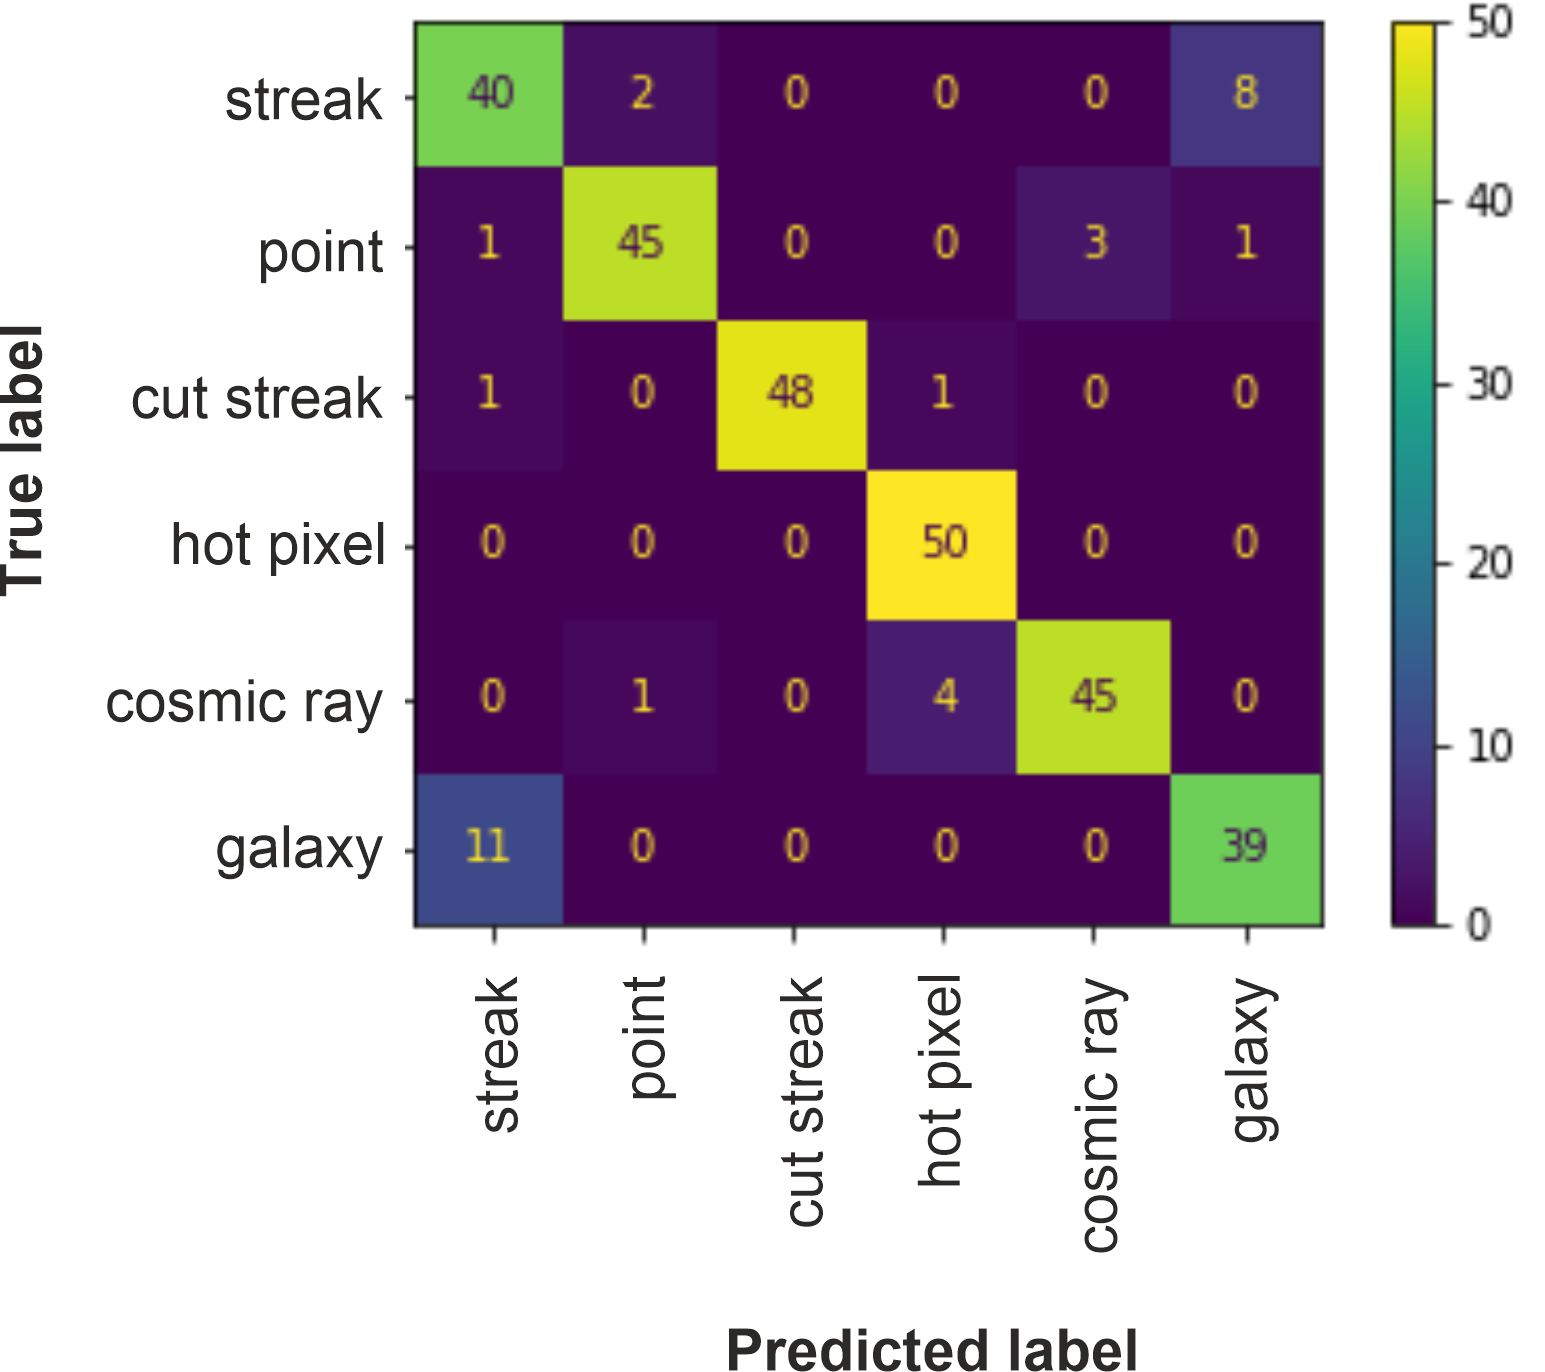
\includegraphics[width=.5\textwidth]{images/confusionMatrix14fe.png}
    \caption{Confusion matrix from the testing of the model with fine-tuned fully-connected layers.}
    \label{img:confmatrixfc}
\end{figure}

\begin{figure}[!h]
\centering
    \begin{subfigure}[t]{.23\textwidth}
        \centering
        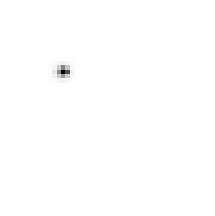
\includegraphics[width=\textwidth]{images/fcwrongImage1.png}
        \caption{}
        \label{fig:pointcosmicmis}
    \end{subfigure}
    \begin{subfigure}[t]{.23\textwidth}
        \centering
        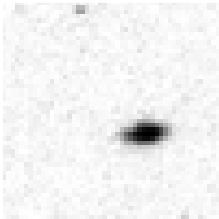
\includegraphics[width=\textwidth]{images/fcwrongImage3.png}
        \caption{}
        \label{fig:galaxylinemis}
    \end{subfigure}
    \begin{subfigure}[t]{.23\textwidth}
        \centering
        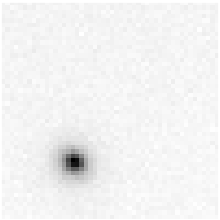
\includegraphics[width=\textwidth]{images/fcwrongImage10.png}
        \caption{}
        \label{fig:pointgalaxymis}
    \end{subfigure}
    \begin{subfigure}[t]{.23\textwidth}
        \centering
        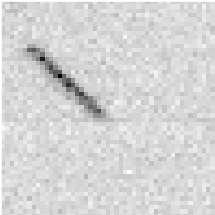
\includegraphics[width=\textwidth]{images/fcwrongImage21.png}
        \caption{}
    \end{subfigure}

    \caption[Wrongly classified images on the model with fine-tuned fully-connected layers.]
    {Wrongly classified images on the model with fine-tuned fully-connected layers. (a) A point misclassified as a cosmic ray, (b) A galaxy misclassified as a streak, (c) A point misclassified as a galaxy, (d) A streak misclassified as a galaxy. }
    \label{fig:wrongfc}
\end{figure}